\documentclass[12pt,a4paper]{article}

% Import basic packages first
\usepackage{tikz}
\usepackage{amsmath, amssymb}
\usepackage{geometry}
\usepackage{xcolor}
\usepackage{hyperref}
\usepackage[most]{tcolorbox}  % Added 'most' option
\usepackage{amsthm}

% Set page geometry
\geometry{margin=1in}

% Define colors
\definecolor{lightblue}{RGB}{173,216,230}
\definecolor{lightgreen}{RGB}{144,238,144}
\definecolor{pastelred}{RGB}{255,182,193}
\definecolor{pastelyellow}{RGB}{255,255,204}

% Define theorem-like environments
\theoremstyle{definition}
\newtheorem{definition}{Definition}[section]
\newtheorem{theorem}[definition]{Theorem}
\newtheorem{property}[definition]{Property}
\newtheorem{example}[definition]{Example}

% Custom box styles
\tcbset{
    theorembox/.style={
        colback=lightblue!10,
        colframe=lightblue!50,
        boxrule=0.5pt,
        left=2mm,
        right=2mm,
        top=1mm,
        bottom=1mm
    }
}

% Title information
\title{\Large\textbf{Graph Theory Visualization}\\[0.5em]
       \normalsize A Visual Guide to Graph Theory Concepts}
\author{\textbf{Ashita Phulwani}\\
        Department of Mathematics}
\date{\today}

\begin{document}

% Title page
\maketitle

% Abstract or Introduction
\begin{tcolorbox}[theorembox]
\begin{abstract}
This document provides visual representations of fundamental graph theory concepts using TikZ. It includes examples of basic graphs, Euler paths, network flows, and spanning trees with detailed explanations and properties.
\end{abstract}
\end{tcolorbox}

\tableofcontents
\newpage

% First section with improved content
\section{Basic Graph Concepts}

\begin{definition}[Graph]
A graph G = (V, E) consists of a set V of vertices and a set E of edges, where each edge connects two vertices.
\end{definition}

\begin{property}[Degree]
The degree of a vertex is the number of edges incident to it.
\end{property}

\begin{center}
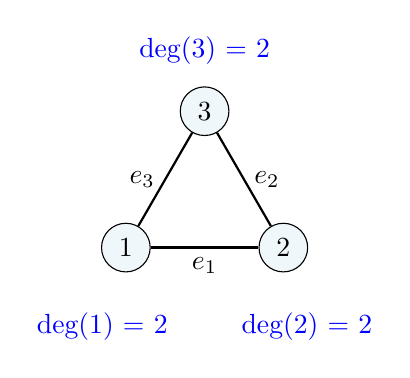
\begin{tikzpicture}
    % Create vertices with labels and degrees
    \node[draw, circle, fill=lightblue!20] (A) at (0,0) {1};
    \node[draw, circle, fill=lightblue!20] (B) at (2,0) {2};
    \node[draw, circle, fill=lightblue!20] (C) at (1,1.732) {3};
    
    % Draw edges with labels
    \draw[thick] (A) -- node[below] {$e_1$} (B);
    \draw[thick] (B) -- node[right] {$e_2$} (C);
    \draw[thick] (C) -- node[left] {$e_3$} (A);
    
    % Add degree annotations
    \node[text=blue] at (-0.3,-1) {deg(1) = 2};
    \node[text=blue] at (2.3,-1) {deg(2) = 2};
    \node[text=blue] at (1,2.5) {deg(3) = 2};
\end{tikzpicture}
\end{center}

\begin{theorem}[Handshaking Lemma]
The sum of degrees of all vertices in a graph is equal to twice the number of edges.
\end{theorem}

\section{Graph Properties}

\begin{tcolorbox}[theorembox]
Important properties of graphs include:
\begin{itemize}
    \item \textbf{Connectivity}: A graph is connected if there exists a path between any two vertices.
    \item \textbf{Planarity}: A graph is planar if it can be drawn without edge crossings.
    \item \textbf{Bipartiteness}: A graph is bipartite if its vertices can be divided into two disjoint sets.
\end{itemize}
\end{tcolorbox}

\begin{example}[Bipartite Graph]
\begin{center}
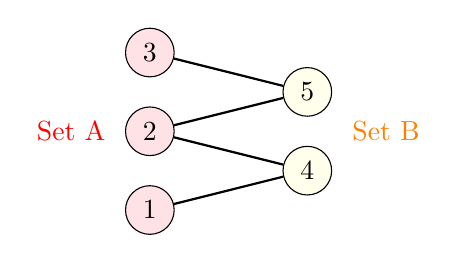
\begin{tikzpicture}
    % Left set vertices
    \node[draw, circle, fill=pastelred!40] (A1) at (0,0) {1};
    \node[draw, circle, fill=pastelred!40] (A2) at (0,1) {2};
    \node[draw, circle, fill=pastelred!40] (A3) at (0,2) {3};
    
    % Right set vertices
    \node[draw, circle, fill=pastelyellow!40] (B1) at (2,0.5) {4};
    \node[draw, circle, fill=pastelyellow!40] (B2) at (2,1.5) {5};
    
    % Draw edges
    \draw[thick] (A1) -- (B1);
    \draw[thick] (A2) -- (B1);
    \draw[thick] (A2) -- (B2);
    \draw[thick] (A3) -- (B2);
    
    % Add set labels
    \node[text=red] at (-1,1) {Set A};
    \node[text=orange] at (3,1) {Set B};
\end{tikzpicture}
\end{center}
\end{example}

\section{Graph Coloring}
\begin{tcolorbox}[theorembox]
A proper vertex coloring is an assignment of colors to vertices such that no adjacent vertices share the same color. The chromatic number \(\chi(G)\) of a graph G is the minimum number of colors needed for a proper coloring.
\end{tcolorbox}

\begin{center}
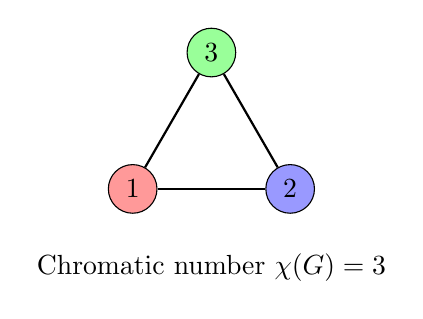
\begin{tikzpicture}
    % Create vertices with different colors
    \node[draw, circle, fill=red!40] (A) at (0,0) {1};
    \node[draw, circle, fill=blue!40] (B) at (2,0) {2};
    \node[draw, circle, fill=green!40] (C) at (1,1.732) {3};
    
    % Draw edges
    \draw[thick] (A) -- (B);
    \draw[thick] (B) -- (C);
    \draw[thick] (C) -- (A);
    
    % Add chromatic number
    \node[text=black] at (1,-1) {Chromatic number \(\chi(G) = 3\)};
\end{tikzpicture}
\end{center}

\begin{property}[Coloring Properties]
For any graph G:
\begin{itemize}
    \item The chromatic number \(\chi(G)\) is at least 2 for any graph with at least one edge
    \item A graph is bipartite if and only if \(\chi(G) = 2\)
    \item For a complete graph K\(_{n}\), \(\chi(K_n) = n\)
\end{itemize}
\end{property}

\section{Special Graph Types}
\begin{tcolorbox}[theorembox]
Common special types of graphs include:
\begin{itemize}
    \item \textbf{Complete Graphs}: Every vertex is connected to every other vertex
    \item \textbf{Cycle Graphs}: A single cycle through all vertices
    \item \textbf{Tree Graphs}: Connected graphs without cycles
\end{itemize}
\end{tcolorbox}

\begin{example}[Complete Graph K4]
\begin{center}
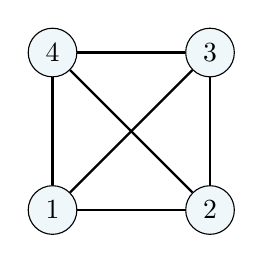
\begin{tikzpicture}
    % Create vertices
    \node[draw, circle, fill=lightblue!20] (A) at (0,0) {1};
    \node[draw, circle, fill=lightblue!20] (B) at (2,0) {2};
    \node[draw, circle, fill=lightblue!20] (C) at (2,2) {3};
    \node[draw, circle, fill=lightblue!20] (D) at (0,2) {4};
    
    % Draw all possible edges
    \draw[thick] (A) -- (B);
    \draw[thick] (B) -- (C);
    \draw[thick] (C) -- (D);
    \draw[thick] (D) -- (A);
    \draw[thick] (A) -- (C);
    \draw[thick] (B) -- (D);
\end{tikzpicture}
\end{center}
\end{example}

\section{Applications}
\begin{tcolorbox}[theorembox]
Graph theory has numerous real-world applications:
\begin{itemize}
    \item \textbf{Network Design}: Communication and transportation networks
    \item \textbf{Schedule Planning}: Course scheduling, resource allocation
    \item \textbf{Social Networks}: Analyzing relationships and connections
    \item \textbf{Circuit Design}: Electronic circuit layout and optimization
\end{itemize}
\end{tcolorbox}

\section{Exercises}
\begin{enumerate}
    \item Find the chromatic number of the complete graph K\(_5\).
    \item Prove that any tree with more than one vertex has chromatic number 2.
    \item Draw a graph with chromatic number 4 that is not a complete graph.
    \item For the bipartite graph shown earlier, verify that its chromatic number is 2.
\end{enumerate}

\section{Conclusion}
\begin{tcolorbox}[theorembox]
Graph theory provides powerful tools for modeling and solving real-world problems. Understanding basic concepts like coloring, connectivity, and special graph types forms the foundation for more advanced applications in computer science, networking, and optimization.
\end{tcolorbox}

\end{document}


